\documentclass[12pt]{article}
\usepackage{amsmath}
\usepackage{graphicx}
\usepackage{hyperref}
\usepackage[ngerman]{babel}
\setlength\parindent{0pt}
\graphicspath{ {./img/} } 


\title{Algorithmen und Komplexität Zusammenfassung}
\author{Fabian Sigmund}
\date{11.07.2023}

\begin{document}
	\maketitle
	\pagebreak
	\section{Sortieralgorithmen (Einfach)}
	\subsection{Selection Sort}
	
	\textbf{a) Sortieren Beispiel:}
	
	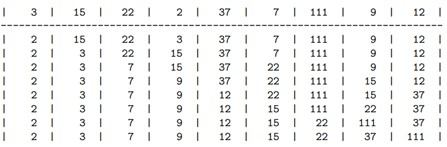
\includegraphics{SelectionSort}
	\break
	
	\textbf{b) Vertausch-Operationen} \hfill \break
	
			\begin{center}
		$Vertausch \ Operationen = Anzahl der Elemente im Array - 1$
	\end{center}
	
	Anmerkung: Selbstvertauschung tritt auf, wenn das jetzige Element schon an der richtigen Stelle ist. Diese müssen per Hand aus der Tabelle von a) ausgelesen werden.
	\newline
	\newline
	\textbf{c) Vergleichs-Operationen}
	\newline
	\newline
	n: Anzahl der Elemente im Array
	
	\begin{center}
		$Vergleichs \ Operationen = $\Large{$\frac{n(n-1)}{2}$}
	\end{center}
	
	Anmerkung: Egal nach welchem Kriterium sortiert wird, diese Formel gilt immer!
	
	\pagebreak
	
	
	\subsection{Insertion Sort}
	\textbf{a) Sortieren Beispiel}
	
	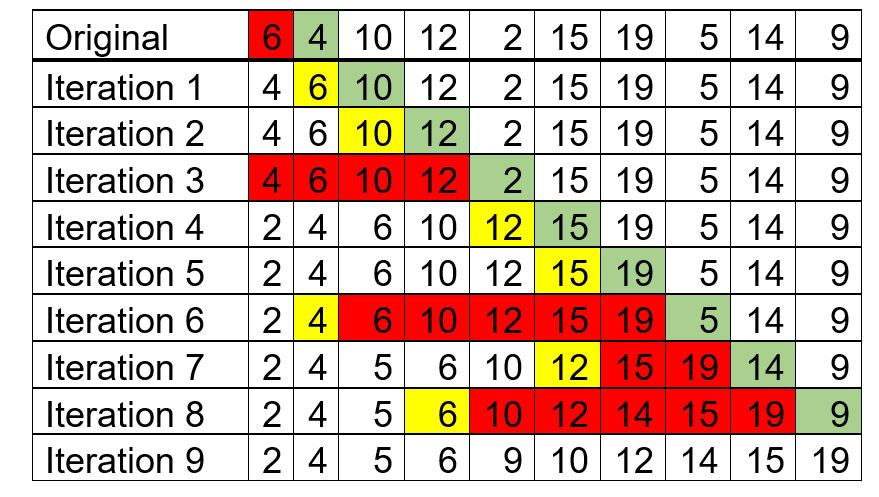
\includegraphics[scale=0.5]{InsertionSort}
	\hfill \break
	
	\textbf{b) Vertausch-Operationen:} \hfill \break
	
	1.	Markiere in jeder Zeile die „Vergleichs-Diagonale grün“
	
	2.	Markiere in jeder Zeile rot bis zum Index auf das grün markierte Element
	
	3.	Vertausch-Operationen = Anzahl der roten Elemente\hfill \break
	
	\textbf{c) Vergleichsoperationen:} \hfill \break
	
	1.	Schritte 1 und 2 von „Vertausch-Operationen“
	
	2.	Markiere, wenn möglich, links ein zusätzliches Kästchen gelb
	
	3.	Vergleichs-Operationen = Anzahl der roten Elemente + Anzahl der gelben Elemente
	
	\newpage
	
	\subsection{Bubble Sort}
	\textbf{a) Sortieren Beispiel}
	\newline\newline
	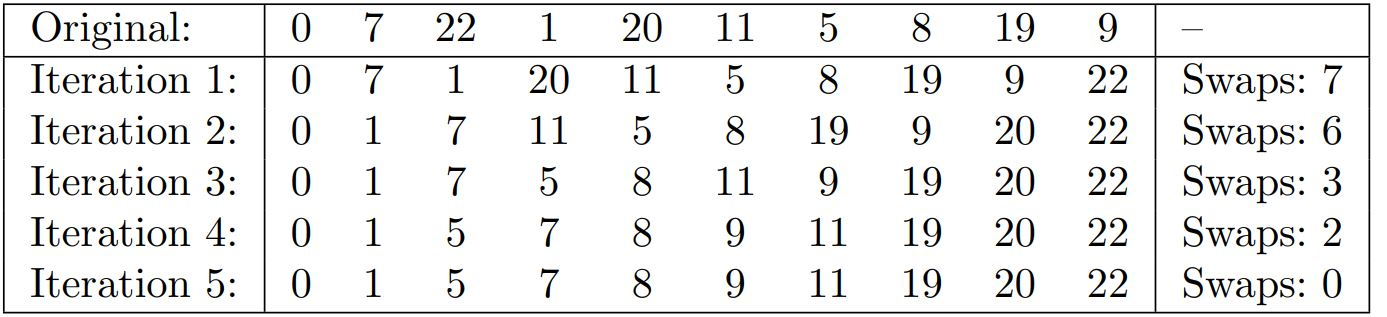
\includegraphics[scale=0.5]{BubbleSort}
	\newline
	
	\textbf{b) Vertausch-Operationen} \newline
	Kein Muster, nur doch durchzählen möglich. \hfill \break
	\newline
	\textbf{c) Vergleichsoperationen}
	

		\begin{center}
		$Vergleichs \ Operationen = selbst geschrieben \ Zeilen * Elemente$
	\end{center}
\newpage
\section{Sortieralgorithmen Divide and Conquer}
\subsection{QuickSort}
\begin{center}
	Original:
\end{center}
\vspace{-0.8cm}
 \begin{center}
 	

 [ 3, 8, 17, 5, 15, 2, 1, 12, 4, 9 ]
 \end{center}
1. Pivotelement wählen und mit dem letzten Element tauschen.
 \begin{center}
	[ 9, 8, 17, 5, 15, 2, 1, 12, 4, (3) ]
\end{center}
2. Von \textbf{links} ausgehend Element suchen, das \textbf{größer} ist als das Pivotelement.

 \begin{center}
	[ \textbf{9}, 8, 17, 5, 15, 2, 1, 12, 4, (3) ]
\end{center}

3. Von \textbf{rechts} ausgehend Element suchen, das \textbf{kleiner} ist als das Pivotelement.

\begin{center}
	[ 9 , 8, 17, 5, 15, 2, \textbf{1}, 12, 4, (3) ]
\end{center}




4. Elemente aus 2. und 3. tauschen
\begin{center}
	[ \textbf{1}, 8, 17, 5, 15, 2, \textbf{9}, 12, 4, (3) ]
\end{center}

5. Schritt 2-4 solange wiederholen bis der Index des Elements aus 2. größer ist als der Index des Elements aus 3.

\begin{center}
	[ \textbf{1}, \textbf{2}, 17, 5, 15, \textbf{8}, \textbf{9}, 12, 4, (3) ]
\end{center}

6. Pivot Element an die richtige stelle zurücktauschen.

\begin{center}
	[ 1, 2, (3), 5, 15, 8 , 9, 12, 4, 17 ]
\end{center}

7. Liste am Pivot Element aufspalten

\begin{center}
	[ 1, 2 ] (3) [ 5, 15, 8 , 9, 12, 4, 17 ]
\end{center}

8. Schritte 1-7 wiederholen bis Liste sortiert ist.
	[(1),  [2]] (3) [4, (5), ]


\end{document}
